\documentclass[8pt,dvipsnames]{beamer}
\usepackage[T1]{fontenc}
\usepackage{libertinus}
\usepackage{amsmath}
\usepackage[most]{tcolorbox}
\usepackage{graphicx}

\usepackage{hyperref}
%python 
\usepackage{listings}
% Default fixed font does not support bold face
\DeclareFixedFont{\ttb}{T1}{txtt}{bx}{n}{8} % for bold
\DeclareFixedFont{\ttm}{T1}{txtt}{m}{n}{8}  % for normal

% Custom colors
\usepackage{color}
\definecolor{deepblue}{rgb}{0,0,0.5}
\definecolor{deepred}{rgb}{0.6,0,0}
\definecolor{deepgreen}{rgb}{0,0.5,0}

\usepackage{listings}

% Python style for highlighting
\newcommand\pythonstyle{\lstset{
		language=Python,
		basicstyle=\ttm,
		morekeywords={self},              % Add keywords here
		keywordstyle=\ttb\color{deepblue},
		emph={MyClass,__init__},          % Custom highlighting
		emphstyle=\ttb\color{deepred},    % Custom highlighting style
		stringstyle=\color{deepgreen},
		frame=tb,                         % Any extra options here
		showstringspaces=false
}}


% Python environment
\lstnewenvironment{python}[1][]
{
	\pythonstyle
	\lstset{#1}
}
{}

% Python for external files
\newcommand\pythonexternal[2][]{{
		\pythonstyle
		\lstinputlisting[#1]{#2}}}

% Python for inline
\newcommand\pythoninline[1]{{\pythonstyle\lstinline!#1!}}

\usepackage{xcolor}  
\newcommand{\cb}[1]{{\color{CadetBlue}#1}}

\usepackage{pgfplots}
\pgfplotsset{compat=newest}
\setlength{\parskip}{0.5em}

\usepackage{setspace}
\setstretch{1.25}  
\usetheme{Singapore}
\setbeamertemplate{navigation symbols}{}


\title{CSE574 Introduction to Machine Learning}
\subtitle{Basic Practice 2}
\author{Jue Guo}
\institute{University at Buffalo}
\date{\today}

\begin{document}
\begin{frame}
	\titlepage
\end{frame}
\begin{frame}
	\frametitle{Outline}
	\tableofcontents
\end{frame}
\section{Learning Algorithm Selection}
\begin{frame}{Learning Algorithm Selection}
	\begin{itemize}
		\item Choosing a machine learning algorithm can be a difficult task. If you have much time, you can try all of them. However, usually the time you have to solve a problem is limited. You can ask yourself several questions before starting to work on the problem. Depending on your answers, you can shortlist some algorithms and try them on your data.
	\end{itemize}
\end{frame}

\begin{frame}
	\textbf{Explainability}
	\begin{itemize}
		\item \textit{Does your model have to be explainable to a non-technical audience? }Most very accurate learning algorithms are so-called "black boxes." They learn models that make very few errors, but why a model made a specific prediction could be very hard to understand and even harder to explain. Examples of such models are neural networks or ensemble models.

		      On the other hand, kNN, linear regression, or decision tree learning algorithms produce models that are not always the most accurate, however, the way they make their prediction is very straightforward.
	\end{itemize}
\end{frame}

\begin{frame}
	\textbf{In-memory vs. out-of-memory}
	\begin{itemize}
		\item Can your dataset be fully loaded into the RAM of your server or personal computer? If yes, then you can choose from a wide variety of algorithms. Otherwise, you would prefer \textbf{incremental learning algorithms} that can improve the model by adding more data gradually.
	\end{itemize}
	\textbf{Number of features and examples}
	\begin{itemize}
		\item How many training examples do you have in your dataset? How many features does each example have? Some algorithms, including \textbf{neural networks} and \textbf{gradient boosting} (we consider both later), can handle a huge number of examples and millions of features. Others, like SVM, can be very modest in their capacity.
	\end{itemize}
\end{frame}

\begin{frame}
	\textbf{Categorical vs. numerical features}
	\begin{itemize}
		\item Is your data composed of categorical only, or numerical only features, or a mix of both? Depending on your answer, some algorithms cannot handle your dataset directly, and you would need to convert your categorical features into numerical ones.
	\end{itemize}
	\textbf{Nonlinearity of the data}
	\begin{itemize}
		\item Is your data linearly separable or can it be modeled using a linear model? If yes, SVM with the linear kernel, logistic or linear regression can be good choices. Otherwise, deep neural networks or ensemble algorithms might work better.
	\end{itemize}
\end{frame}

\begin{frame}
	\textbf{Training Speed}
	\begin{itemize}
		\item How much time is a learning algorithm allowed to use to build a model? Neural networks are known to be slow to train. Simple algorithms like logistic and linear regression or decision trees are much faster. Specialized libraries contain very efficient implementations of some algorithms; you may prefer to do research online to find such libraries. Some algorithms, such as random forests, benefit from the availability of multiple CPU cores, so their model building time can be significantly reduced on a machine with dozens of cores.
	\end{itemize}
\end{frame}

\begin{frame}
	\textbf{Prediction Speed}
	\begin{itemize}
		\item How fast does the model have to be when generating predictions? Will your model be used in production where very high throughput is required? Algorithms like SVMs, linear and logistic regression, and (some types of) neural networks, are extremely fast at the prediction time. Others, like kNN, ensemble algorithms, and very deep or recurrent neural networks, are slower.

		      If you don't want to guess the best algorithm for your data, a popular way to choose one is by testing it on the validation set. We talk about that below. Alternatively, if you use scikit-learn, you could try their algorithm selection diagram.
	\end{itemize}
\end{frame}

\begin{frame}
	\begin{figure}
		\centering
		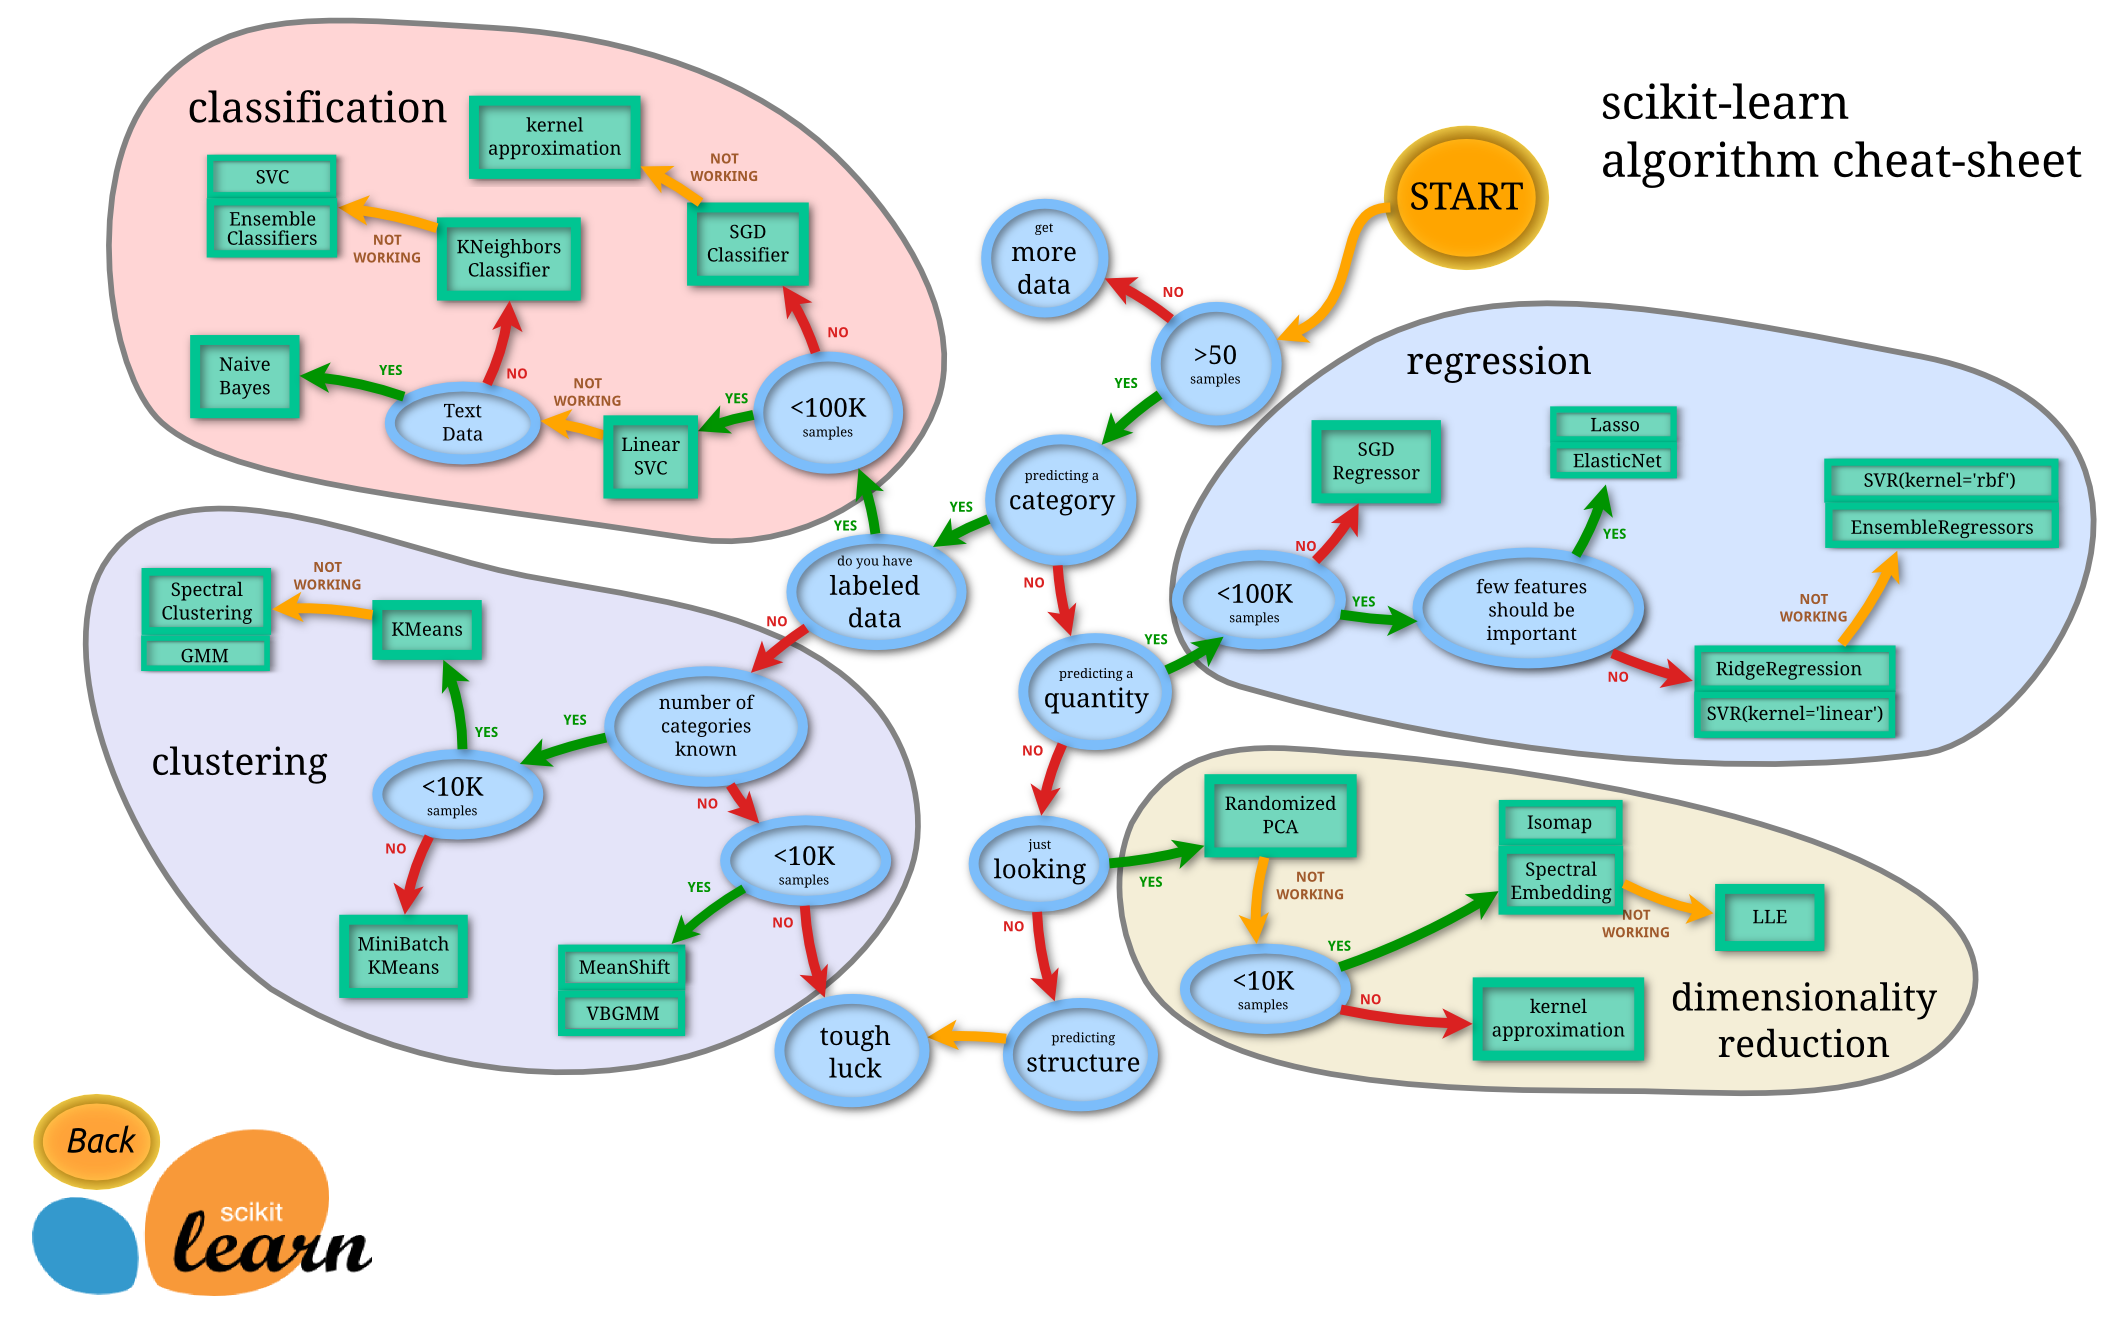
\includegraphics[width=\textwidth]{imgs/Basic_Practice_1.png}
	\end{figure}
\end{frame}

\section{Three Sets}
\begin{frame}{Three Sets}
	I used the expression ``dataset" and ``training set" interchangeably, However, in practice data analysts work with three distinct sets of labeled examples:
	\begin{enumerate}
		\item training set,
		\item validation set, and
		\item test set.
	\end{enumerate}
	Once you have got your annotated dataset, the first thing you do is you shuffle the examples and split the dataset into three subsets: \textbf{training}, \textbf{validation}, and \textbf{test}. The training set is usually the biggest one; you use it to build the model. The validation and test sets are roughly the same sizes, much smaller than the size of the training set. The learning algorithm cannot use examples from these two subsets to build the model. That is why those two sets are often called \textbf{holdout sets}.
\end{frame}
\begin{frame}
	Something to be aware of:
	\begin{itemize}
		\item There's no optimal proportion to split the dataset into these three subsets. In the past, the rule of thumb was to use $70 \%$ of the dataset for training, $15 \%$ for validation and $15 \%$ for testing. However, in the age of big data, datasets often have millions of examples. In such cases, it could be reasonable to keep $95 \%$ for training and 2.5\%/2.5\% for validation/testing.
		\item You may wonder, what is the reason to have three sets and not one. The answer is simple: when we build a model, what we do not want is for the model to only do well at predicting labels of examples the learning algorithms has already seen. A trivial algorithm that simply memorizes all training examples and then uses the memory to "predict" their labels will make no mistakes when asked to predict the labels of the training examples, but such an algorithm would be useless in practice. What we really want is a model that is good at predicting examples that the learning algorithm didn't see: weant good performance on a holdout set.
	\end{itemize}
\end{frame}
\begin{frame}
	\textbf{Why do we need two holdout sets and not one? }
	\begin{itemize}
		\item We use the validation set to
		      \begin{enumerate}
			      \item choose the learning algorithm, and
			      \item  find the best values of hyperparameters.
		      \end{enumerate}
		      We use the test set to assess the model before delivering it to the client or putting it in production.
	\end{itemize}
\end{frame}

\section{Underfitting and Overfitting}
\begin{frame}{Underfitting and Overfitting}
	I mentioned above the notion of \textbf{bias}. I said that a model has a low bias if it predicts well the labels of the training data. If the model makes many mistakes on the training data, we say that the model has a \textbf{high bias} or that the model \textbf{underfits}. So, underfitting is the inability of the model to predict well the labels of the data it was trained on. There could be several reasons for underfitting, the most important of which are:
	\begin{itemize}
		\item your model is too simple for the data (for example a linear model can often underfit);
		\item the features you engineered are not informative enough.
	\end{itemize}
	\begin{figure}
		\centering
		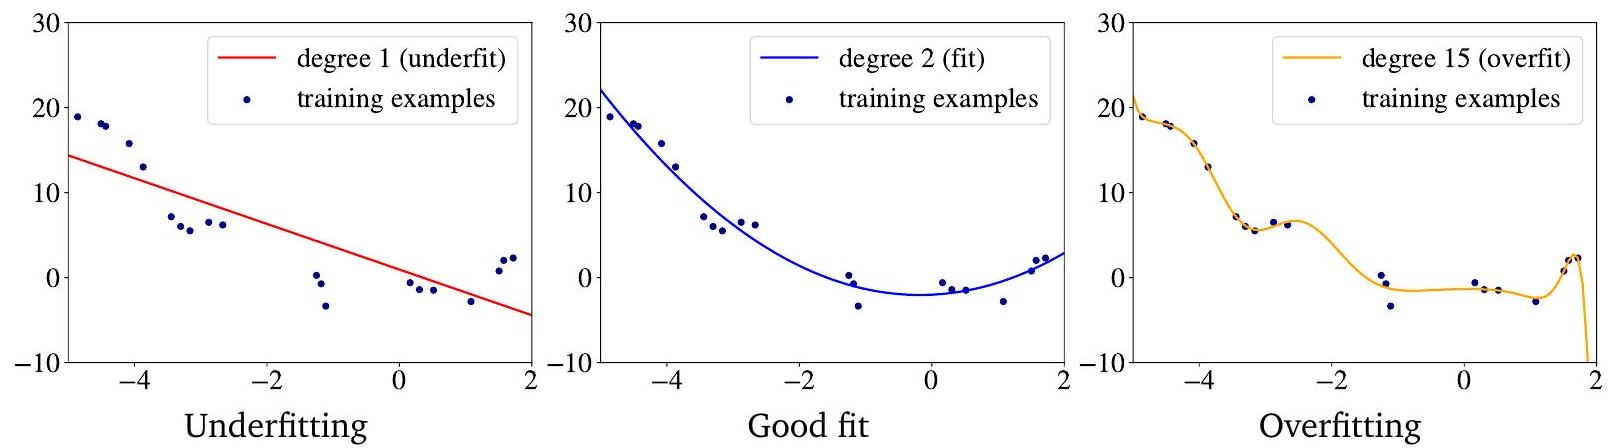
\includegraphics[width=0.7\textwidth]{imgs/Basic_Practice_2.jpeg}
		\caption{Examples of underfitting (linear model), good fit (quadratic model), and overfitting (polynomial of degree 15).}
	\end{figure}
\end{frame}

\begin{frame}
	The \textit{first reason} is easy to illustrate in the case of one-dimensional regression: the dataset can resemble a curved line, but our model is a straight line. The \textit{second reason} can be illustrated like this: let's say you want to predict whether a patient has cancer, and the features you have are height, blood pressure, and heart rate. These three features are clearly not good predictors for cancer so our model will not be able to learn a meaningful relationship between these features and the label.
	\begin{itemize}
		\item The solution to the problem of underfitting is to try a more complex model or to engineer features with higher predictive power.
	\end{itemize}
\end{frame}

\begin{frame}
	\textbf{Overfitting} is another problem a model can exhibit. \textit{The model that overfits predicts very well the training data but poorly the data from at least one of the two holdout sets.}  Several reasons can lead to overfitting, the most important of which are:
	\begin{itemize}
		\item your model is too complex for the data (for example a very tall decision tree or a very deep or wide neural network often overfit);
		\item you have too many features but a small number of training examples.
	\end{itemize}
	In the literature, you can find another name for the problem of overfitting: the problem of \textbf{high variance}. This term comes from statistics. The variance is an error of the model due to its sensitivity to small fluctuations in the training set. \textit{It means that if your training data was sampled differently, the learning would result in a significantly different model.} Which is why the model that overfits performs poorly on the test data: test and training data are sampled from the dataset independently of one another.
\end{frame}

\begin{frame}
	Even the \underline{simplest} model, such as linear, can overfit the data.
	\begin{itemize}
		\item That usually happens when the data is high-dimensional, but the number of training examples is relatively low.
	\end{itemize}
	In fact, when feature vectors are very high-dimensional, the linear learning algorithm can build a model that assigns non-zero values to most parameters $w^{(j)}$ in the parameter vector $\mathbf{w}$, trying to find very complex relationships between all available features to predict labels of training examples perfectly.

	Such a \underline{complex} model will most likely predict poorly the labels of the holdout examples. This is because by trying to perfectly predict labels of all training examples, the model will also learn the idiosyncrasies of the training set: \textit{the noise in the values of features of the training examples, the sampling imperfection due to the small dataset size, and other artifacts extrinsic to the decision problem at hand but present in the training set}.
\end{frame}

\begin{frame}
	Several solutions to the problem of overfitting are possible:
	\begin{enumerate}
		\item Try a simpler model (linear instead of polynomial regression, or SVM with a linear kernel instead of RBF, a neural network with fewer layers/units).
		\item Reduce the dimensionality of examples in the dataset (for example, by using one of the dimensionality reduction techniques \textit{discuss in future sessions}).
		\item Add more training data, if possible.
		\item Regularize the model.
	\end{enumerate}
	\textbf{Regularization} is the most widely used approach to prevent overfitting.
\end{frame}

\section{Regularization}
\begin{frame}{Regularization}
	\textbf{Regularization} is an umbrella term that encompasses methods that force the learning algorithm to build a less complex model. In practice, that often leads to slightly higher bias but significantly reduces the variance. This problem is known in the literature as the \textbf{bias-variance tradeoff}.
	\begin{itemize}
		\item The two most widely used types of regularization are called $\mathbf{L 1}$ and $\mathbf{L 2}$ \textbf{regularization}. The idea is quite simple. To create a regularized model, we modify the objective function by adding a penalizing term whose value is higher when the model is more complex.
	\end{itemize}
\end{frame}

\begin{frame}
	For simplicity, I illustrate regularization using the example of linear regression. The same principle can be applied to a wide variety of models.
	Recall the linear regression objective:

	$$
		\min _{\mathbf{w}, b} \frac{1}{N} \sum_{i=1}^{N}\left(f_{\mathbf{w}, b}\left(\mathbf{x}_{i}\right)-y_{i}\right)^{2}
	$$
\end{frame}

\begin{frame}
	An \textit{L1-regularized objective (Lasso Regression)} looks like this:

	$$
		\min _{\mathbf{w}, b}\left[C|\mathbf{w}|+\frac{1}{N} \sum_{i=1}^{N}\left(f_{\mathbf{w}, b}\left(\mathbf{x}_{i}\right)-y_{i}\right)^{2}\right]
	$$

	where $|\mathbf{w}| \stackrel{\text { def }}{=} \sum_{j=1}^{D}\left|w^{(j)}\right|$ and $C$ is a hyperparameter that controls the importance of regularization.
	\begin{itemize}
		\item If we set $C$ to zero, the model becomes a standard non-regularized linear regression model. On the other hand, if we set to $C$ to a high value, the learning algorithm will try to set most $w^{(j)}$ to a very small value or zero to minimize the objective, and the model will become very simple which can lead to underfitting.
	\end{itemize}
	Your role as the data analyst is to find such a value of the hyperparameter $C$ that doesn't increase the bias too much but reduces the variance to a level reasonable for the problem at hand.
\end{frame}

\begin{frame}
	An \textit{L2-regularized objective (Ridge Regression)} looks like this:

	$$
		\min _{\mathbf{w}, b}\left[C\|\mathbf{w}\|^{2}+\frac{1}{N} \sum_{i=1}^{N}\left(f_{\mathbf{w}, b}\left(\mathbf{x}_{i}\right)-y_{i}\right)^{2}\right], \text { where }\|\mathbf{w}\|^{2} \stackrel{\text { def }}{=} \sum_{j=1}^{D}\left(w^{(j)}\right)^{2}
	$$

	In practice, L1 regularization produces a \textbf{sparse model}, a model that has most of its parameters (in case of linear models, most of $w^{(j)}$ ) equal to zero, provided the hyperparameter $C$ is large enough.
	\begin{itemize}
		\item So L1 performs \textbf{feature selection} by deciding which features are essential for prediction and which are not. That can be useful in case you want to increase model explainability.
	\end{itemize}
	However, if your only goal is to maximize the performance of the model on the holdout data, then L2 usually gives better results. L2 also has the advantage of being differentiable, so gradient descent can be used for optimizing the objective function.
\end{frame}

\begin{frame}
	L1 and L2 regularization methods were also combined in what is called \textbf{elastic net regularization} with L1 and L2 regularizations being special cases. You can find in the literature the name \textbf{ridge regularization }for L2 and \textbf{lasso} for L1.

	In addition to being widely used with linear models, L1 and L2 regularization are also frequently used with neural networks and many other types of models, which directly minimize an objective function.

	Neural networks also benefit from two other regularization techniques: \textbf{dropout} and \textbf{batch-normalization}. There are also non-mathematical methods that have a regularization effect: \textbf{data augmentation} and \textbf{early stopping}.
\end{frame}

\begin{frame}{Think ... \textbf{5 mins} }
	Consider the vector \(\vec{x}=(1, \varepsilon) \in \mathbb{R}^{2}\) where \(\varepsilon>0\) is small. The \(l_{1}\)
	and \(l_{2}\) norms of \(\vec{x}\), respectively, are given by
	$$
		\|\vec{x}\|_{1}=1+\varepsilon,\|\vec{x}\|_{2}^{2}=1+\varepsilon^{2}
	$$
	Now say that, as part of some regularization procedure, we are
	going to reduce the magnitude of one of the elements of \(\vec{x}\) by \(\delta \leq \varepsilon\)
	. If we change \(x_{1}\) to \(1-\delta\), the resulting norms are
	$$
		\|\vec{x}-(\delta, 0)\|_{1}=1-\delta+\varepsilon,\|\vec{x}-(\delta, 0)\|_{2}^{2}=1-2 \delta+\delta^{2}+\varepsilon^{2}
	$$
	On the other hand, reducing \(x_{2}\) by \(\delta\) gives norms
	$$
		\|\vec{x}-(0, \delta)\|_{1}=1-\delta+\varepsilon,\|\vec{x}-(0, \delta)\|_{2}^{2}=1-2 \varepsilon \delta+\delta^{2}	+\varepsilon^{2}
	$$
\end{frame}

\begin{frame}{What did you notice?}
	The thing to notice here is that, for an \(l_{2}\) penalty, regularizing the larger term \(x_{1}\) results in a much greater reduction in norm than doing so to the smaller term \(x_{2} \approx 0\). For the \(l_{1}\) penalty, however, the reduction is the same.
	\begin{itemize}
		\item when penalizing a model using the \(l_{2}\) norm, it is highly unlikely that anything will ever be set to zero, since the reduction in \(l_{2}\) norm going from \(\epsilon\) to \(0\) is almost nonexistent when \(\epsilon\) is small.
		\item On the other hand, the reduction in \(l_{1}\) norm is always equal to \(\delta\), regardless of the quantity being penalized.
	\end{itemize}
	Another way to think of it: it's not so much that \(l_{1}\) penalties encourage sparsity, but that \(l_{2}\) penalties in some sense discourage sparsity by yielding diminishing returns as elements are moved closer to zero.
\end{frame}

\section{Model Performance Assessment}
\begin{frame}{Model Performance Assessment}
	Once you have a model which our learning algorithm has built using the training set, how can you say how good the model is? You use the test set to assess the model.

	The test set contains the examples that the learning algorithm has never seen before, so if our model performs well on predicting the labels of the examples from the test set, we say that our model \textbf{generalizes well} or, simply, that it's good.
\end{frame}

\begin{frame}
	To be more rigorous, machine learning specialists use various formal metrics and tools to assess the model performance.
	\begin{itemize}
		\item For regression, the assessment of the model is quite simple. A well-fitting regression model results in predicted values close to the observed data values.
		\item The \textbf{mean model}, which always predicts the average of the labels in the training data, generally would be used if there were no informative features.
	\end{itemize}
	The fit of a regression model being assessed should, therefore, be better than the fit of the mean model. If this is the case, then the next step is to compare the performances of the model on the training and the test data.
\end{frame}

\begin{frame}
	To do that, we compute the mean squared error (MSE) for the training, and, separately, for the test data. If the MSE of the model on the test data is substantially higher than the MSE obtained on the training data, this is a sign of overfitting. Regularization or a better hyperparameter tuning could solve the problem. The meaning of "substantially higher" depends on the problem at hand and has to be decided by the data analyst jointly with the decision maker/product owner who ordered the model. For classification, things are a little bit more complicated. The most widely used metrics and tools to assess the classification model are:
	\begin{itemize}
		\item confusion matrix,
		\item accuracy,
		\item cost-sensitive accuracy,
		\item precision/recall, and
		\item area under the ROC curve.
	\end{itemize}
	To simplify the illustration, I use a binary classification problem. Where necessary, I show how to extend the approach to the multiclass case.
\end{frame}

\subsection{Confusion Matrix}
\begin{frame}{Confusion Matrix}
	The \textbf{confusion matrix }is a table that summarizes how successful the classification model is at predicting examples belonging to various classes.
	\begin{itemize}
		\item One axis of the confusion matrix is the label that the model predicted, and the other axis is the actual label. In a binary classification problem, there are two classes.
	\end{itemize}
	Let's say, the model predicts two classes: "spam" and "not\_spam":

	\begin{center}
		\begin{tabular}{lll}
			\hline               & spam (predicted)  & not\_spam (predicted) \\
			\hline spam (actual) & $23(\mathrm{TP})$ & $1(\mathrm{FN})$      \\
			not\_spam (actual)   & $12(\mathrm{FP})$ & $556(\mathrm{TN})$    \\
			\hline
		\end{tabular}
	\end{center}

\end{frame}

\begin{frame}{Confusion Matrix: Binary Classification}
	The notation can be confusing but repeat several times and it will make sense
	\begin{center}
		\begin{tabular}{lll}
			\hline               & spam (predicted)  & not\_spam (predicted) \\
			\hline spam (actual) & $23(\mathrm{TP})$ & $1(\mathrm{FN})$      \\
			not\_spam (actual)   & $12(\mathrm{FP})$ & $556(\mathrm{TN})$    \\
			\hline
		\end{tabular}
	\end{center}

	The above confusion matrix shows that of the 24 examples that actually were spam, the model correctly classified 23 as spam.
	\begin{itemize}
		\item In this case, we say that we have 23 \textbf{true positives} or $\mathrm{TP}=23$. The model incorrectly classified 1 example as not\_spam.In this case, we have 1 \textbf{false negative}, or $\mathrm{FN}=1$.
		\item Similarly, of 568 examples that actually were not spam, 556 were correctly classified (556 \textbf{true negatives} or $\mathrm{TN}=556)$, and 12 were incorrectly classified ( 12 \textbf{false positives}, $\mathrm{FP}=12$ ).
	\end{itemize}
\end{frame}

\begin{frame}{Confusion Matrix: Multiclass Classification}
	The confusion matrix for multiclass classification has as many rows and columns as there are different classes. It can help you to determine mistake patterns.
	\begin{itemize}
		\item For example, a confusion matrix could reveal that a model trained to recognize different species of animals tends to mistakenly predict "cat" instead of "panther," or "mouse" instead of "rat." In this case, you can decide to add more labeled examples of these species to help the learning algorithm to "see" the difference between them.
	\end{itemize}
	Alternatively, you might add additional features the learning algorithm can use to build a model that would better distinguish between these species. Confusion matrix is used to calculate two other performance metrics: \textbf{precision} and \textbf{recall}.
\end{frame}
\subsection{Percision/Recall}
\begin{frame}{Percision/Recall}
	The two most frequently used metrics to assess the model are \textbf{precision} and \textbf{recall}. Precision is the ratio of correct positive predictions to the overall number of positive predictions:

	$$
		\text { precision } \stackrel{\text { def }}{=} \frac{\mathrm{TP}}{\mathrm{TP}+\mathrm{FP}} \text {. }
	$$

	Recall is the ratio of correct positive predictions to the overall number of positive examples in the dataset:

	$$
		\text { recall } \stackrel{\text { def }}{=} \frac{\mathrm{TP}}{\mathrm{TP}+\mathrm{FN}} \text {. }
	$$
\end{frame}

\begin{frame}{}
	To understand the meaning and importance of precision and recall for the model assessment it is often useful to think about the prediction problem as the problem of research of documents in the database using a query.
	\begin{itemize}
		\item The precision is the proportion of relevant documents in the list of all returned documents.
		\item The recall is the ratio of the relevant documents returned by the search engine to the total number of the relevant documents that could have been returned.
	\end{itemize}
	In the case of the spam detection problem, we want to have high precision (we want to avoid making mistakes by detecting that a legitimate message is spam) and we are ready to tolerate lower recall (we tolerate some spam messages in our inbox).
\end{frame}

\begin{frame}
	Almost always, in practice, we have to choose between a high precision or a high recall. It's usually impossible to have both. We can achieve either of the two by various means:
	\begin{itemize}
		\item by assigning a higher weighting to the examples of a specific class (the SVM algorithm accepts weightings of classes as input);
		\item by tuning hyperparameters to maximize precision or recall on the validation set;
		\item by varying the decision threshold for algorithms that return probabilities of classes; for instance, if we use logistic regression or decision tree, to increase precision (at the cost of a lower recall), we can decide that the prediction will be positive only if the probability returned by the model is higher than 0.9.
	\end{itemize}
	Even if precision and recall are defined for the binary classification case, you can always use it to assess a multiclass classification model.
	\begin{itemize}
		\item 	To do that, first select a class for which you want to assess these metrics. Then you consider all examples of the selected class as positives and all examples of the remaining classes as negatives.
	\end{itemize}
\end{frame}

\subsection{Accuracy}
\begin{frame}{Accuracy}
	\textbf{Accuracy} is given by the number of correctly classified examples divided by the total number of classified examples. In terms of the confusion matrix, it is given by:

	$$
		\text { accuracy } \stackrel{\text { def }}{=} \frac{\mathrm{TP}+\mathrm{TN}}{\mathrm{TP}+\mathrm{TN}+\mathrm{FP}+\mathrm{FN}} \text {. }
	$$
	Accuracy is a useful metric when errors in predicting all classes are equally important. In case of the spam/not spam, this may not be the case.
	\begin{itemize}
		\item 	For example, you would tolerate false positives less than false negatives. A false positive in spam detection is the situation in which your friend sends you an email, but the model labels it as spam and doesn't show you.
		\item On the other hand, the false negative is less of a problem: if your model doesn't detect a small percentage of spam messages, it's not a big deal.
	\end{itemize}
\end{frame}

\subsection{Area under the ROC Curve (AUC)}
\begin{frame}{Area under the ROC Curve (AUC)}
	The ROC curve (stands for "receiver operating characteristic;" the term comes from radar engineering) is a commonly used method to assess the performance of classification models. ROC curves use a combination of the \textbf{true positive rate} (defined exactly as \textbf{recall}) and false positive rate (the proportion of negative examples predicted incorrectly) to build up a summary picture of the classification performance.

	The true positive rate (TPR) and the false positive rate (FPR) are respectively defined as,

	$$
		\mathrm{TPR} \stackrel{\text { def }}{=} \frac{\mathrm{TP}}{\mathrm{TP}+\mathrm{FN}} \text { and } \mathrm{FPR} \stackrel{\text { def }}{=} \frac{\mathrm{FP}}{\mathrm{FP}+\mathrm{TN}}
	$$

	ROC curves can only be used to assess classifiers that return some confidence score (or a probability) of prediction. For example, logistic regression, neural networks, and decision trees (and ensemble models based on decision trees) can be assessed using ROC curves.
\end{frame}

\begin{frame}
	\begin{enumerate}
		\item To draw a ROC curve, you first discretize the range of the confidence score. If this range for a model is $[0,1]$, then you can discretize it like this: $[0,0.1,0.2,0.3,0.4,0.5,0.6,0.7,0.8,0.9,1]$.
		\item Then, you use each discrete value as the prediction threshold and predict the labels of examples in your dataset using the model and this threshold.
	\end{enumerate}
	For example, if you want to compute TPR and FPR for the threshold equal to 0.7, you apply the model to each example, get the score, and, if the score is higher than or equal to 0.7 , you predict the positive class; otherwise, you predict the negative class.
\end{frame}

\begin{frame}
	Look at the illustration.
	\begin{itemize}
		\item We can see that if the threshold is \(0\), all our predictions will be positive, so both TPR and FPR will be 1 (the upper right corner).
		\item On the other hand, if the threshold is \(1\), then no positive prediction will be made, both TPR and FPR will be zero which corresponds to the lower left corner.
	\end{itemize}

	\begin{figure}
		\centering
		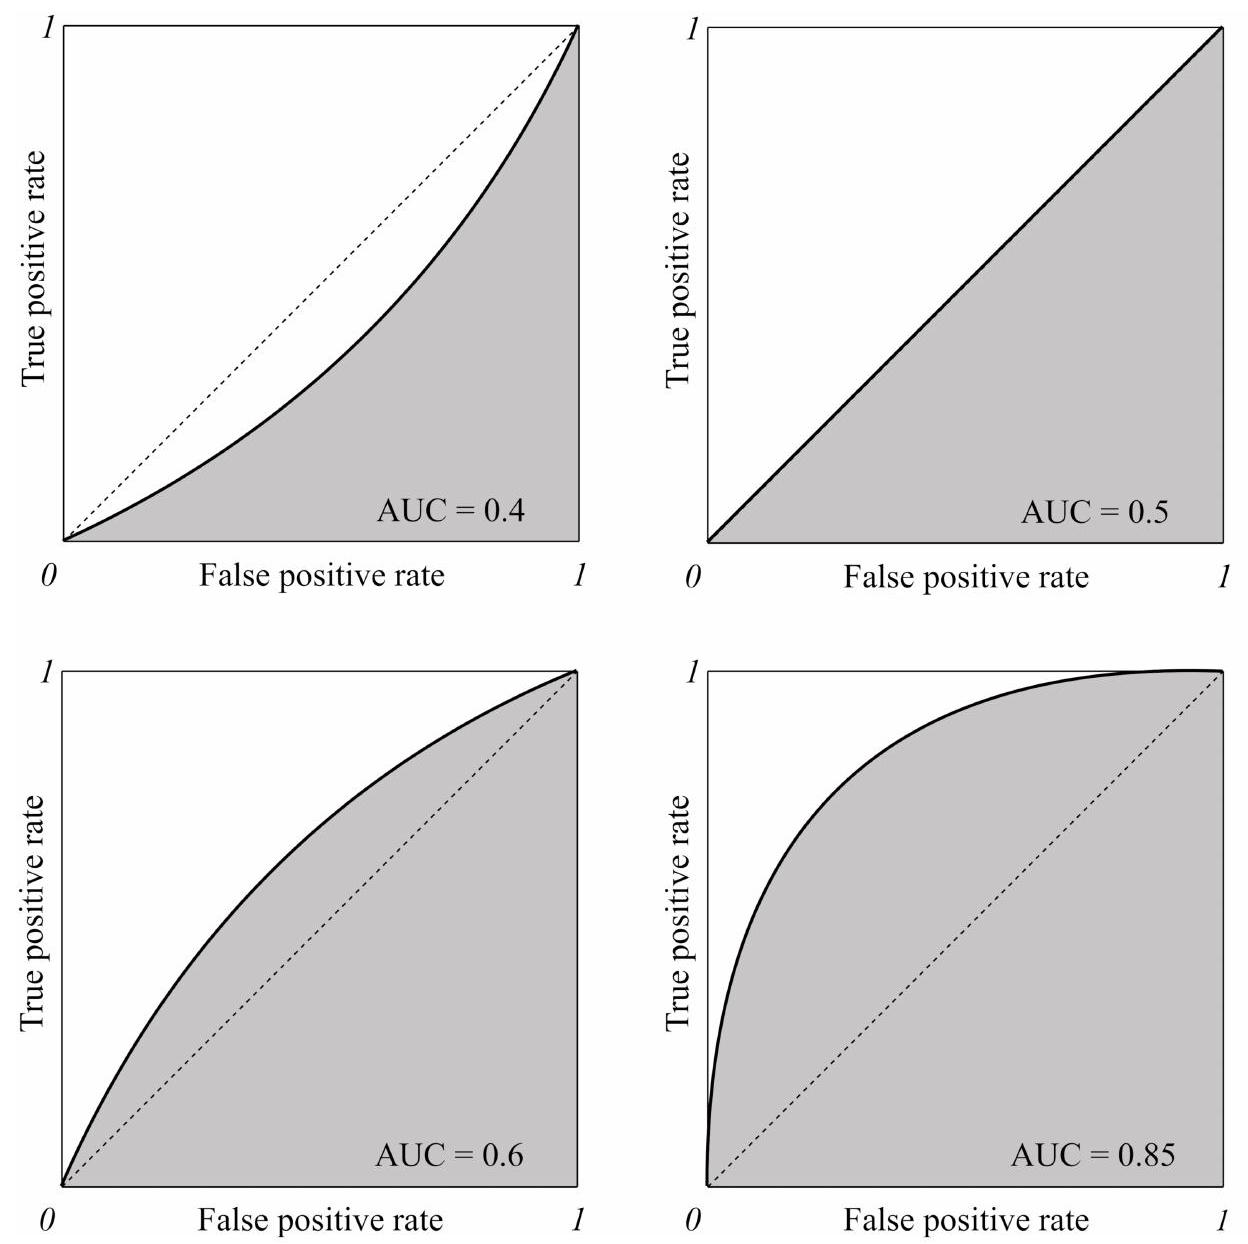
\includegraphics[width=0.4\textwidth]{imgs/Basic_Practice_3.jpeg}
		\caption{The area under the ROC curve (shown on gray).}
	\end{figure}
\end{frame}

\begin{frame}
	\begin{figure}
		\centering
		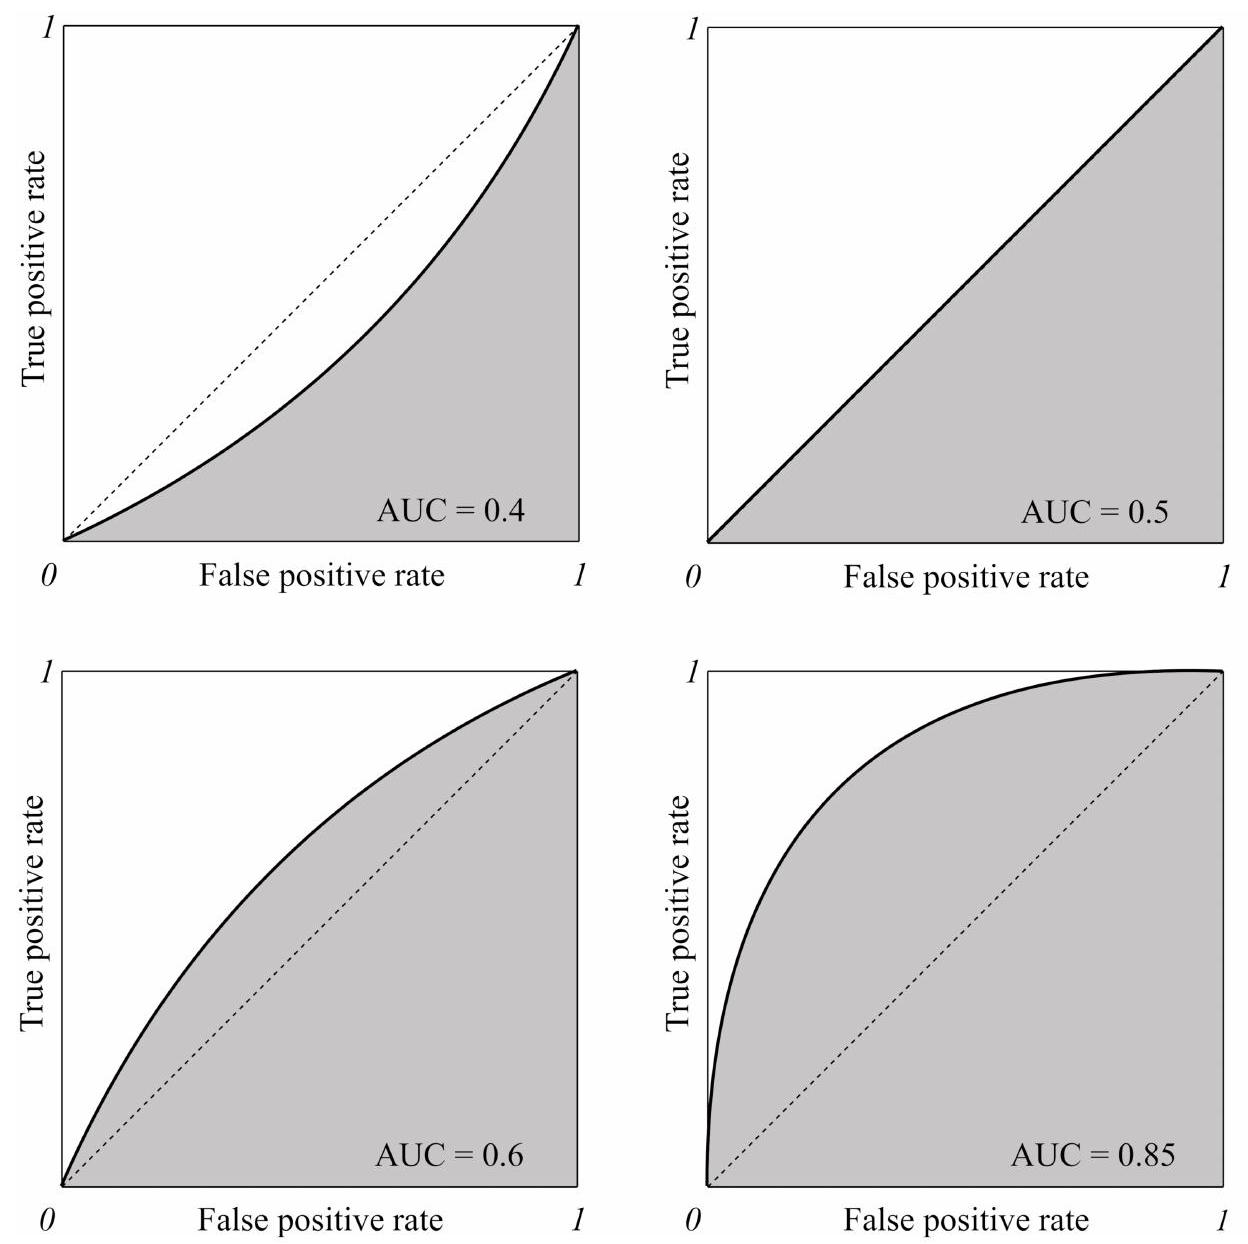
\includegraphics[width=0.4\textwidth]{imgs/Basic_Practice_3.jpeg}
		\caption{The area under the ROC curve (shown on gray).}
	\end{figure}
	The higher \textbf{the area under the ROC curve} (AUC), the better the classifier. A classifier with an AUC higher than 0.5 is better than a random classifier. If AUC is lower than 0.5, then something is wrong with your model. A perfect classifier would have an AUC of 1. Usually, if your model behaves well, you obtain a good classifier by selecting the value of the threshold that gives TPR close to 1 while keeping FPR near 0.
\end{frame}

\begin{frame}
	ROC curves are popular because they are relatively simple to understand, they capture more than one aspect of the classification (by taking both false positives and negatives into account) and allow visually and with low effort comparing the performance of different models.
\end{frame}

\section{Hyperparameter Tuning}
\begin{frame}{Hyperparameter Tuning}
	When I presented learning algorithms, I mentioned that you as a data analyst have to select good values for the algorithm's hyperparameters, such as $\epsilon$ and $d$ for ID3, $C$ for SVM, or $\alpha$ for gradient descent.
	\begin{itemize}
		\item As you already know, hyperparameters aren't optimized by the learning algorithm itself. The data analyst has to "tune" hyperparameters by experimentally finding the best combination of values, one per hyperparameter.
	\end{itemize}
	One typical way to do that, when you have enough data to have a decent validation set (in which each class is represented by at least a couple of dozen examples) and the number of hyperparameters and their range is not too large is to use \textbf{grid search}.
\end{frame}
\begin{frame}{Grid Search}
	Grid search is the most simple \textbf{hyperparameter tuning} technique. Let's say you train an SVM and you have two hyperparameters to tune: the penalty parameter $C$ (a positive real number) and the kernel (either "linear" or "rbf").
	\begin{itemize}
		\item If it's the first time you are working with this particular dataset, you don't know what is the possible range of values for $C$. The most common trick is to use a logarithmic scale. For example, for $C$ you can try the following values: [0.001, 0.01, 0.1, 1, 10, 100, 1000]. In this case you have 14 combinations of hyperparameters to try: [(0.001, "linear"), (0.01, "linear"), (0.1, "linear"), (1, "linear"), (10, "linear"), (100, "linear"), (1000, "linear"), (0.001, "rbf"), (0.01, "rbf"), (0.1, "rbf"), (1, "rbf"), (10, "rbf"), (100, "rbf"), (1000, "rbf")].
		\item You use the training set and train 14 models, one for each combination of hyperparameters. Then you assess the performance of each model on the validation data using one of the metrics we discussed in the previous section (or some other metric that matters to you). Finally, you keep the model that performs the best according to the metric.
	\end{itemize}
	Once the best pair of hyperparameters is found, you can try to explore the values close to the best ones in some region around them. Sometimes, this can result in an even better model. Finally, you assess the selected model using the test set.
\end{frame}

\begin{frame}{Other Techniques}
	As you could notice, trying all combinations of hyperparameters, especially if there are more than a couple of them, could be time-consuming, especially for large datasets. There are more efficient techniques, such as \textbf{random search} and \textbf{Bayesian hyperparameter optimization}.
	\begin{itemize}
		\item Random search differs from grid search in that you no longer provide a discrete set of values to explore for each hyperparameter; instead, you provide a statistical distribution for each hyperparameter from which values are randomly sampled and set the total number of combinations you want to try.
		\item Bayesian techniques differ from random or grid search in that they use past evaluation results to choose the next values to evaluate. The idea is to limit the number of expensive optimizations of the objective function by choosing the next hyperparameter values based on those that have done well in the past.
	\end{itemize}
\end{frame}
\subsection{Cross-Validation}
\begin{frame}{Cross-Validation}
	When you don't have a decent validation set to tune your hyperparameters on, the common technique that can help you is called \textbf{cross-validation}. When you have few training examples, it could be prohibitive to have both validation and test set. You would prefer to use more data to train the model. In such a case, you only split your data into a training and a test set. Then you use cross-validation on the training set to simulate a validation set.

	Cross-validation works as follows.
	\begin{enumerate}
		\item First, you fix the values of the hyperparameters you want to evaluate.
		\item Then you split your training set into several subsets of the same size. Each subset is called a fold. Typically, five-fold cross-validation is used in practice. With five-fold cross-validation, you randomly split your training data into five folds: $\left\{F_{1}, F_{2}, \ldots, F_{5}\right\}$. Each $F_{k}, k=1, \ldots, 5$ contains $20 \%$ of your training data.
	\end{enumerate}
\end{frame}

\begin{frame}
	Then you train five models as follows.
	\begin{enumerate}[3.]
		\item To train the first model, $f_{1}$, you use all examples from folds $F_{2}, F_{3}, F_{4}$, and $F_{5}$ as the training set and the examples from $F_{1}$ as the validation set.
		\item To train the second model, $f_{2}$, you use the examples from folds $F_{1}, F_{3}, F_{4}$, and $F_{5}$ to train and the examples from $F_{2}$ as the validation set.
	\end{enumerate}
	You continue building models iteratively like this and compute the value of the metric of interest on each validation set, from $F_{1}$ to $F_{5}$. Then you average the five values of the metric to get the final value.

	You can use grid search with cross-validation to find the best values of hyperparameters for your model. Once you have found these values, you use the entire training set to build the model with these best values of hyperparameters you have found via cross-validation. Finally, you assess the model using the test set.
\end{frame}
\end{document}